\documentclass[tikz,border=3pt]{standalone}
\usepackage{amsmath,amssymb}\usepackage{mathptmx}
\usepackage{tikz}
\usetikzlibrary{arrows.meta,positioning,fit,backgrounds,calc,shapes.geometric,decorations.pathreplacing}
\definecolor{ink}{HTML}{1F1F1E}
\definecolor{muted}{HTML}{5F5E58}
\definecolor{base}{HTML}{F3F3F1}
\definecolor{baseedge}{HTML}{8A8980}
\definecolor{newc}{HTML}{CDE2FB}
\definecolor{newedge}{HTML}{1C5CAB}
\definecolor{accent}{HTML}{EB6834}
\definecolor{accentlt}{HTML}{FBE1D6}
\tikzset{
  >={Stealth[length=2.2mm]},
  blk/.style={draw=baseedge, fill=base, rounded corners=2pt, align=center, font=\footnotesize,
              minimum height=10mm, inner sep=3pt, line width=0.5pt},
  newblk/.style={blk, draw=newedge, fill=newc, line width=0.8pt},
  accblk/.style={blk, draw=accent, fill=accentlt, line width=0.8pt},
  flow/.style={->, draw=ink, line width=0.6pt},
  newflow/.style={->, draw=newedge, line width=0.8pt, dashed},
  lbl/.style={font=\scriptsize, text=muted, align=center},
}

\begin{document}
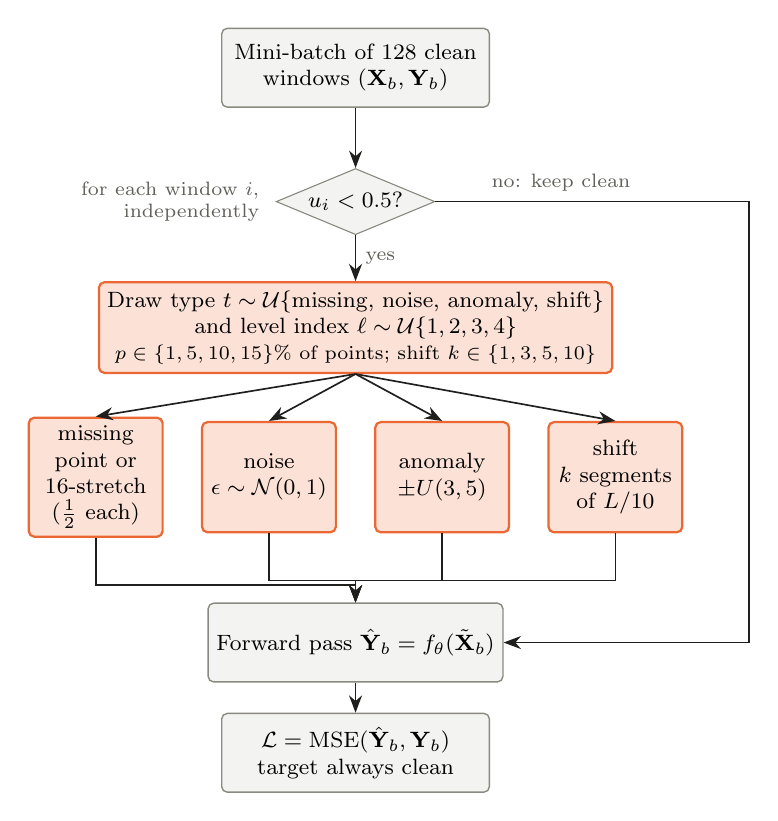
\begin{tikzpicture}
  \node[blk, minimum width=34mm] (b) at (0,0) {Mini-batch of 128 clean\\windows $(\mathbf{X}_b,\mathbf{Y}_b)$};
  \node[diamond, aspect=2.4, draw=baseedge, fill=base, font=\footnotesize, inner sep=1pt] (d) at (0,-1.7) {$u_i<0.5$?};
  \node[accblk, minimum width=50mm] (typ) at (0,-3.3) {Draw type $t\sim\mathcal{U}\{\text{missing, noise, anomaly, shift}\}$\\and level index $\ell\sim\mathcal{U}\{1,2,3,4\}$\\{\scriptsize $p\in\{1,5,10,15\}\%$ of points;\ shift $k\in\{1,3,5,10\}$}};
  \node[accblk, minimum width=17mm, minimum height=14mm] (m) at (-3.3,-5.2) {missing\\point or\\16-stretch\\($\tfrac12$ each)};
  \node[accblk, minimum width=17mm, minimum height=14mm] (n) at (-1.1,-5.2) {noise\\$\epsilon\sim\mathcal{N}(0,1)$};
  \node[accblk, minimum width=17mm, minimum height=14mm] (a) at (1.1,-5.2) {anomaly\\$\pm U(3,5)$};
  \node[accblk, minimum width=17mm, minimum height=14mm] (s) at (3.3,-5.2) {shift\\$k$ segments\\of $L/10$};
  \node[blk, minimum width=34mm] (f) at (0,-7.3) {Forward pass $\hat{\mathbf{Y}}_b=f_\theta(\tilde{\mathbf{X}}_b)$};
  \node[blk, minimum width=34mm] (l) at (0,-8.7) {$\mathcal{L}=\text{MSE}(\hat{\mathbf{Y}}_b,\mathbf{Y}_b)$\\target always clean};
  \draw[flow] (b) -- (d);
  \draw[flow] (d) -- node[lbl, right] {yes} (typ);
  \draw[flow] (d.east) -- (5.0,-1.7) node[lbl, above, pos=0.4] {no: keep clean} |- (f.east);
  \foreach \x in {m,n,a,s} { \draw[flow] (typ.south) -- (\x.north); \draw[flow] (\x.south) -- ++(0,-0.6) -| (f.north); }
  \draw[flow] (f) -- (l);
  \node[lbl, align=right, anchor=east] at (-1.1,-1.7) {for each window $i$,\\independently};
\end{tikzpicture}
\end{document}
